% Generated from main.typ. Typst is authoritative; regeneration overwrites this file.
\documentclass{qlnotes-export}

\title{Math 525: Probability}
\subtitle{Typst-first course notes}
\author{Qiulin Fan}
\date{2026}

\begin{document}
\mainmatter
\chapter{basic combinatorics and probability space}\label{basic-combinatorics-and-probability-space}

\section{permutations and combinations}\label{permutations-and-combinations}

\subsection{permutations}\label{permutations}

\begin{definition}{\protect\phantomsection\label{kn-permutations}{\textbf{permutations}}}

一个 permutation 就是对一组 objects 的一个 \textbf{rearrangement} (这些 objects 中可以有 same 的也可以有 distinct 的).\\
对于 \(n\) 个 \textbf{distinct objects}, 一共存在

\[n! = n(n - 1)(n - 2)\cdots\]

个 permutations.

\end{definition}

\begin{example}

求 "STATISTICS" 的 \# distinct permutations.

\end{example}

\begin{qlsolution}{Solution}

这里一共有 10 个 objects. 但问题是: 其中有 3 个 \(S\), 3 个 \(T\), 2 个 \(I\) 是相同的.\\
于是: 我们首先假设它们都是 distinct 的, 则存在 \(10!\) 个 permutations. 而, 每个 permutation 都包含了对 3 个 \(S\) 的一个子 permutation. 而对 3 个 \(S\) 的任意 permutation 都是相同的! 同样的道理 apply to 3 个 \(T\) 和 2 个 \(I\).\\
所以这个结果是真实结果的 \(3!3!2!\) 倍.\\
同样地, 由于 因而, 正确结果是:

\[\frac{10!}{3!3!2!1!1!}\]

\end{qlsolution}

\begin{qlremark}{Remark}

求一组 objects 的 distinct permutations 的数量时, 对于其中相同的 objects, 我们只需要除去它们的重复数量的 factorial (即: 它们自己内部有多少个 permutation 都算作一个 permutation).\\
公式:

\[\frac{n!}{n_{1}!n_{2}!\cdots n_{k}!}\]

其中 \(n_{1},n_{2},\cdots,n_{k}\) 是每个 object 的重复数量.\\
这个式子又叫做 multinomial coefficient.

\begin{definition}{\protect\phantomsection\label{kn-multinomial-coefficient}{\textbf{multinomial
coefficient}}}

令 \(n \in {\mathbb{N}},n_{1},n_{2},\cdots,n_{k} \in {\mathbb{N}},n_{1} + n_{2} + \cdots + n_{k} = n\), 我们定义 multinomial coefficient:

\[\left( \frac{n}{n_{1},n_{2},\cdots,n_{k}} \right) = \frac{n!}{n_{1}!n_{2}!\cdots n_{k}!}\]

\end{definition}

\begin{proposition}

如果我们需要 \(n_{1}\) 个 object 1, \(n_{2}\) 个 object 2, \(\cdots\), \(n_{k}\) 个 object \(k\), 那么它们的 distinct permutations 的数量为:

\[\left( \frac{n_{1} + n_{2} + \cdots + n_{k}}{n_{1},n_{2},\cdots,n_{k}} \right)\]

\end{proposition}

\end{qlremark}

\subsection{combinations}\label{combinations}

\begin{definition}{\protect\phantomsection\label{kn-combinations}{\textbf{combinations}}}

一个 combination 就是从一个 set 中选取若干个 elements, 而忽略它们的顺序.

\end{definition}

\begin{proposition}

从 \(n\) 个 \textbf{distinct objects} 中选取 \(k\) 个的 combinations 的数量为:

\[\left( \frac{n}{k} \right) = \frac{n!}{k!(n - k)!}\]

\end{proposition}

\begin{proof}

我们可以将问题转化为: 从 \(n\) 个 \textbf{distinct objects} 中选取 \(k\) 个的 permutations 的数量, 然后再除去重复的 permutations. 而, 从 \(n\) 个 \textbf{distinct objects} 中选取 \(k\) 个的 permutations 的数量为:

\[n \times (n - 1) \times \cdots \times (n - k + 1) = \frac{n!}{(n - k)!}\]

而其中, 对于每个 valid combination, 都包含了它的所有 ordered permutations, 即重复了 \(k!\) 次. 因此, 最终的结果为:

\[\frac{n!}{k!(n - k)!}\]

\end{proof}

\subsection{binomial theorem}\label{binomial-theorem}

\begin{theorem}{\protect\phantomsection\label{kn-binomial-theorem}{\textbf{Binomial
Theorem}}}

令 \(x,y \in {\mathbb{R}},n \in {\mathbb{N}}\), 则有:

\[(x + y)^{n} = \sum\limits_{k = 0}^{n}\left( \frac{n}{k} \right)x^{n - k}y^{k}\]

\end{theorem}

\begin{proof}

我们可以 prove this by combiinatorial interpretation. 因为把 \(x + y\) 展开即 \(n\) 个 \((x + y)\) 的乘积. 即: 对于每个被乘项, 我们都是在 \(x\) 和 \(y\) 之间选择一个.\\
因而: \(x^{k}y^{n - k}\) 的系数就是从 \(n\) 个 \((x + y)\) 中选取 \(k\) 个 \(x\) 的 combinations 的数量, 即 \(\left( \frac{n}{k} \right)\).\\
考虑所有的 possible \(k\) 值, 我们得到:

\[(x + y)^{n} = \sum\limits_{k = 0}^{n}\left( \frac{n}{k} \right)x^{n - k}y^{k}\]

这是 combinatorial 的 proof.

\end{proof}

另外一种更轮椅的思路是 prove by induction. 这需要一个辅助的 proposition:

\begin{proposition}

\[\left( \frac{n}{k} \right) = \left( \frac{n - 1}{k - 1} \right) + \left( \frac{n - 1}{k} \right)\]

\end{proposition}

这个等式的 combinatorial interpretation 很 trivial: 对于其中的任意一个 object:

\begin{itemize}
\item
  这个 object 被选中的情况, combinations 的数量: \(\left( \frac{n - 1}{k - 1} \right)\) (从其他里面选 \(k - 1\) 个);
\item
  这个 object 不被选中的情况, combinations 的数量: \(\left( \frac{n - 1}{k} \right)\) (从其他里面选 \(k\) 个).
\end{itemize}

\begin{example}

一个 52-card deck, 取 5 张随机牌, 我们获得:

\begin{itemize}
\item
  4 张同 rank 的牌, 最后一张不同 rank 的牌
\item
  a full house (3 张同 rank 的牌, 2 张同 rank 的牌)
\end{itemize}

的概率是多少?

\end{example}

\begin{qlsolution}{Solution}

一共有 \(\left( \frac{52}{5} \right)\) 种取法. 取 4 张同 rank 的牌: 13 种取法. 取最后一张不同 rank 的牌: 52-4 = 48 种取法. 因而, 概率是:

\[\frac{13 \times 48}{\left( \frac{52}{5} \right)}\]

如果是取 3 张同 rank 的牌 + 两张 different 同 rank 的牌: 我们首先在 4 个花色里面选 3 个, 有 \(\left( \frac{4}{3} \right)\) 种取法.\\
因而选取 3 cards of the same rank 的数量为: \(13 \cdot \left( \frac{4}{3} \right)\).\\
然后选取剩余的两张: 然后故技重施, 从剩下的 12 个 rank 里面选 1 个, 而选择它们的花色有 \(\left( \frac{4}{2} \right)\) 种取法. 因而, 概率是:

\[\frac{13 \cdot \left( \frac{4}{3} \right) \cdot 12 \cdot \left( \frac{4}{2} \right)}{\left( \frac{52}{5} \right)}\]

\end{qlsolution}

\begin{example}

我们有 \(n\) 把钥匙, 其中有一把是正确的. 尝试 \(k\) 次, 能够成功开门的概率是多少?

\end{example}

\begin{qlsolution}{Solution}

一共有 \(n!\) 种钥匙的 permutations. 我们需要的情况: 正确的钥匙出现在前 \(k\) 个位置:

\begin{itemize}
\item
  正确钥匙出现在第 \(1\) 个位置, 其他 \(n - 1\) 随便排列: \(\cdot (n - 1)!\) 种
\item
  \(\cdots\)
\item
  正确钥匙出现在第 \(k\) 个位置, 其他 \(n - 1\) 随便排列: \(k \cdot (n - 1)!\) 种
\end{itemize}

因而正确的 permutations 的数量为:

\[k \cdot (n - 1)!\]

因而, 概率是:

\[\frac{k \cdot (n - 1)!}{n!} = \frac{k}{n}\]

\end{qlsolution}

\begin{qlremark}{Remark}

正确钥匙出现在每个位置上的概率都是 \(1/n\). 因而它出现在前 \(k\) 个位置的概率就是 \(k/n\).\\
这是一类典型的问题: 不放回的抽取. 在只关心"是否在前 \(k\) 次成功"这一事件时, 这个过程等价于"正确钥匙在一个随机排列中的位置". 这一结果只和比例有关, 与过程细节无关. 只要没有信息bias, 没有偏好, 完全随机, 那么成功概率只取决于:

\begin{itemize}
\item
  你允许的尝试次数 \(k\)
\item
  总可能性数 \(n\)
\end{itemize}

而如果是放回则是不同的情况. 通过补事件容易得:

\[{\mathbb{P}}(A) = 1 - \left( {1 - \frac{1}{n}} \right)^{k}\]

放回和不防回最大的区别是: 放回时, 每次尝试都是独立的, 而不放回时, 每次尝试都不是独立的. 最明显的例子就是, 如果不放回, \(k = n\) 时概率为 1. 而如果放回, 不论 \(k\) 有多大, 概率都小于 1; 当 \(k \ll n\) 的时候, 这两个概率相近 (符合直觉, 因为 \(n\) 很大时放回和不放回几乎没区别.)

\end{qlremark}

\begin{example}

一个篮子里有 \(10\) 个 red balls 和 \(5\) 个 blue balls. 我们随机从中取出 \(3\) 个 balls, exactly 其中 \(1\) 个是 blue ball 的概率是多少? 如果每次都放回呢?

\end{example}

\begin{qlsolution}{Solution}

不放回:

\[{\mathbb{P}}(\text{exactly one blue ball}) = \left( \frac{10}{2} \right)\left( \frac{5}{1} \right)\ \ \left( \frac{15}{3} \right) = \frac{45}{91}\]

放回: 5 ways to choose the blue ball, 10 ways to choose the red ball, 以及 3 positions to place the blue ball,

\[{\mathbb{P}}(\text{exactly one blue ball}) = 3 \cdot \frac{3 \cdot 10^{2}}{15^{3}}\]

\end{qlsolution}

\subsection{combinations with repetition}\label{combinations-with-repetition}

\begin{definition}{\protect\phantomsection\label{kn-combinations-with-repetition}{\textbf{combinations
with repetition}}}

一个 combination with repetition 就是从一个 set 中选取若干个 elements, 而忽略它们的顺序, 并且\textbf{允许重复选取}.

\end{definition}

\begin{proposition}

从 \(n\) 个 \textbf{distinct objects} 中选取 \(k\) 个的 combinations with repetition 的数量为:

\[\left( \frac{n + k - 1}{k} \right)\]

\end{proposition}

\begin{qlremark}{Remark}

关于这个问题我们最开始可能会犯一个错误: 认为 combinations with \(k\) repetitions 的数量为:

\[\left( \frac{kn}{k} \right)\]

但是想一下就知道这是错的. 因为我们相当于给 repeated 的同一个 objects 赋予了顺序, 从而计入了额外的数量.

\end{qlremark}

\begin{proof}

这个问题比较巧妙. 我们上面错误的尝试已经表明: 用 "make copies" 的方法行不通. 我们需要变换一下思路. 原问题是 "要选哪几个元素, 每个元素要选几个". 而我们可以把这个问题理解为: 一共有 \(k\) 个位置, \(n\) 个组, 我们给每个组分配多少个位置?\\
Formalize 这个想法即: 对于第 \(i\) 个 object, 我们给它分配 \(x_{i}\) 个位置. 所有满足条件的 combinations 可以 represent by:

\[\left\{ {y = (x_{1},x_{2},\cdots,x_{n}) \in {\mathbb{Z}}_{\geq 0}^{n}:x_{1} + x_{2} + \cdots + x_{n} = k} \right\}\]

到这里我们想到一个经典的问题: stars and bars. 即: 把 \(k\) 个星星分成 \(n\) 个组, 每个组至少有 1 个星星. 这个问题等价于: 把 \(k\) 个星星和 \(n - 1\) 个隔板排成一排, 然后选择 \(n - 1\) 个隔板的位置.\\
问题是: 我们这里, 一个组可以有 \(0\) 个 stars; 但是这是小问题. 因为我们可以 set \(x_{i}' = x_{i} + 1\), 问题等价转化为:

\[\left\{ {y = (x_{1}',x_{2}',\cdots,x_{n}') \in {\mathbb{Z}}_{\geq 1}^{n}:x_{1}' + x_{2}' + \cdots + x_{n}' = k + n} \right\}\]

这就强制每个组至少有一个 star, 于是可以使用 stars and bars 的方法来解决. 即: 用 \(n - 1\) 个隔板隔开 \(k + n\) 个星星 (有 \(k + n - 1\) 个空档). 因而, 满足条件的 combinations 的数量为:

\[\left( \frac{k + n - 1}{n - 1} \right) = \left( \frac{k + n - 1}{k} \right)\]

\end{proof}

\begin{example}

有 5 种口味的 ice creams. 一个人随机选择 20 个 scoops. 求: 每种口味至少被选中一次的 probability.

\end{example}

\begin{qlsolution}{Solution}

即从 \(5\) 种口味中选取 \(20\) 个 combinations with repetition. 于是 sample space 的大小: \(\left( \frac{25 - 1}{20} \right)\).\\
而满足条件的 combinations: 即每种口味我们都预选一个. 然后再从\(5\) 种口味中选取 \(15\) 个 combinations with repetition.

\[{\mathbb{P}}(\text{each flavor is selected at least once}) = \frac{\left( \frac{19}{15} \right)}{\left( \frac{24}{20} \right)} = \frac{\left( \frac{24}{20} \right)}{\left( \frac{24}{20} \right)}\]

\end{qlsolution}

\subsection{inclusion-exclusion principle}\label{inclusion-exclusion-principle}

\begin{proposition}{\protect\phantomsection\label{kn-inclusion-exclusion-principle}{\textbf{inclusion-exclusion
principle}}}

如果 \(\Omega\) 是 \href{https://qiulinfan.github.io/qlblog/notes/math/measure-theory/\#kn-measure-space}{measure space} 意义下的一个 finite measure space, 那么对于任意 \(A_{1},\ldots,A_{n} \subseteq \Omega\) 的, 有:

\[\left| {\cup_{i = 1}^{n}A_{i}} \right| = \sum\limits_{i = 1}^{n}\left| A_{i} \right| - \sum\limits_{i < j}\left| {A_{i} \cap A_{j}} \right| + \sum\limits_{i < j < k}\left| {A_{i} \cap A_{j} \cap A_{k}} \right| - \ldots + ( - 1)^{n + 1}\left| {A_{1} \cap \ldots \cap A_{n}} \right|.\]

\end{proposition}

\begin{qlremark}{Remark}

这里的 \(\sum_{i < j}\) 等 index 意思就是\textbf{考虑所有可能的 combinations}, 不考虑顺序, 和下标的顺序没有关系. 比如一共有三个集合 \(A_{1},A_{2},A_{3}\), 那么 \(\left. \sum_{i < j} \middle| A_{i} \cap A_{j}| \right.\) 就是 \(A_{1} \cap A_{2},A_{1} \cap A_{3},A_{2} \cap A_{3}\) 的并集.\\
这个定理是 countable additivity 的直接推广.

\end{qlremark}

\begin{example}

(Divisibility) 令 \(n \in {\mathbb{N}}\), 我们随机取一个 \(x \in \left\{ {1,2,\cdots,n} \right\}\), 求 \(x\) is divisible by 2 or 3 or 5 的概率.

\end{example}

\begin{qlsolution}{Solution}

令 \(A_{2},A_{3},A_{5}\) 为 \(x\) 是 2, 3, 5 的倍数的 events. 即:

\[A_{i} = \left\{ {k \in \left\{ {1,2,\cdots,n} \right\} \mid k\ \text{is divisible by}\ i} \right\}\]

于是我们要计算的是:

\[\begin{matrix}
{{\mathbb{P}}(A_{2} \cup A_{3} \cup A_{5})} & {= {\mathbb{P}}(A_{2}) + {\mathbb{P}}(A_{3}) + {\mathbb{P}}(A_{5}) - {\mathbb{P}}(A_{2} \cap A_{3}) - {\mathbb{P}}(A_{2} \cap A_{5}) - {\mathbb{P}}(A_{3} \cap A_{5}) + {\mathbb{P}}(A_{2} \cap A_{3} \cap A_{5})} \\
 & {= \frac{\lfloor\frac{n}{2}\rfloor + \lfloor\frac{n}{3}\rfloor + \lfloor\frac{n}{5}\rfloor - \lfloor\frac{n}{6}\rfloor - \lfloor\frac{n}{10}\rfloor - \lfloor\frac{n}{15}\rfloor + \lfloor\frac{n}{30}\rfloor}{n}}
\end{matrix}\]

\end{qlsolution}

\begin{example}[(matching problem)]

假设有 \(n\) 个人参加一个 event, 每个人都上交了一顶帽子; 现在再把帽子随机地发给每个人, 求没有人拿回自己的帽子的概率.

\begin{qlsolution}{Solution}

令 \(A_{i}\) 为第 \(i\) 个人拿回自己的帽子的事件. 则我们要求的概率是: \({\mathbb{P}}(\bigcap_{i = 1}^{n}A_{i}^{c})\).

\[\begin{matrix}
{{\mathbb{P}}(\bigcap\limits_{i = 1}^{n}A_{i}^{c})} & {= {\mathbb{P}}((\bigcup\limits_{i = 1}^{n}A_{i})^{c})} \\
 & {= 1 - {\mathbb{P}}(\bigcup\limits_{i = 1}^{n}A_{i})} \\
 & {= 1 - \frac{|\bigcup_{i = 1}^{n}A_{i}|}{n!}}
\end{matrix}\]

由于:

\[\begin{matrix}
{|\bigcup\limits_{i = 1}^{n}A_{i}|} & {= \sum\limits_{i = 1}^{n}\left| A_{i} \right| - \sum\limits_{i < j}\left| {A_{i} \cap A_{j}} \right| + \sum\limits_{i < j < k}\left| {A_{i} \cap A_{j} \cap A_{k}} \right| - \ldots + ( - 1)^{n + 1}\left| {A_{1} \cap \ldots \cap A_{n}} \right|} \\
 & {= \left( \frac{n}{1} \right)(n - 1)! - \left( \frac{n}{2} \right)(n - 2)! + \left( \frac{n}{3} \right)(n - 3)! - \cdots + ( - 1)^{n + 1}} \\
 & {= n!\sum\limits_{k = 1}^{n}( - 1)^{k - 1}\frac{1}{k!}}
\end{matrix}\]

我们可以得到:

\[{\mathbb{P}}(\bigcap\limits_{i = 1}^{n}A_{i}^{c}) = \sum\limits_{k = 2}^{n}\frac{( - 1)^{k}}{k!}\]

\end{qlsolution}

\end{example}

\begin{qlremark}{Remark}

当 \(k\rightarrow\infty\) 的时候, 这个结果趋向于 \(e^{- 1} \approx 0.367879\). (By Taylor's expansion of \(e^{x}\).)

\end{qlremark}

\section{probability space}\label{probability-space}

我们这里跳过所有 measure theory 的内容, 见 notes on measure theory.\\

\begin{definition}{\protect\phantomsection\label{kn-probability-space}{\textbf{probability
space}} ,
\protect\phantomsection\label{kn-probability-measure}{\textbf{probability
measure}} ,
\protect\phantomsection\label{kn-sample-space}{\textbf{sample space}} ,
\protect\phantomsection\label{kn-event-space}{\textbf{event space}}}

按 \href{https://qiulinfan.github.io/qlblog/notes/math/measure-theory/\#kn-measure-space}{measure space} 的定义, 一个 probability space 是三元组 \((\Omega,\mathcal{F},{\mathbb{P}})\), 其中 \({\mathbb{P}}(\varnothing) = 0,{\mathbb{P}}(\Omega) = 1\).\\
对于这样的 \href{https://qiulinfan.github.io/qlblog/notes/math/measure-theory/\#kn-measure}{measure} \(\mathbb{P}\), 我们称之为 \textbf{probability measure (概率测度, 即概率)}.\\
而这里的 \(\Omega\) 我们称之为 \textbf{sample space (样本空间)}; 这里的 \href{https://qiulinfan.github.io/qlblog/notes/math/measure-theory/\#kn-sigma-algebra}{\(\sigma\)-algebra} \(\mathcal{F}\), 我们称之为 \textbf{event space (事件空间)}.\\
任意的 \(A \subset \Omega\) 都是一个 \textbf{event}, 但是概率论中只考虑 \(A \in \mathcal{F}\), 即 measurable event. 为简化, event 这个单词就指 measurable event.

\end{definition}

\begin{qlremark}{Remark}

回顾一下 measure space 的定义:

\begin{itemize}
\item
  一个 set \(\Omega\) 的一个 \(\sigma\)-algebra 就是一个包含空集的子集簇, 其 \textbf{closed under countable unions and complements}. (如果只 closed under finite unions, 则只称为一个 algebra.)
\item
  一个 Borel algebra 是一个定义在 topological space 上的 \(\sigma\)-algebra, 由 all open sets 生成. (因而: closed under countable unions and complements.) \(\mathbb{R}\) 的 Borel algebra 可以由 all open intervals 生成.
\item
  一个 measure on a measurable space \((\Omega,\mathcal{F})\) 就是一个从 \(\mathcal{F}\rightarrow{\mathbb{R}}\) 的函数, 满足 \textbf{countable additivity}.
\item
  measure 的性质: \textbf{(1)non-negativity, (2) monotonicity, (3) countable subadditivity, (4) inclusion-exclusion principle (上节已讲), (5) continuity from below and above.} 第 (5) 条具体即: For measurable sets \(A_{1} \subseteq A_{2} \subseteq \cdots \subseteq A_{n} \subseteq \cdots\), then \(\lim_{n\rightarrow\infty}{\mathbb{P}}(A_{n}) = {\mathbb{P}}(\bigcup_{n = 1}^{\infty}A_{n})\).\\
  For measurable sets \(A_{1} \supseteq A_{2} \supseteq \cdots \supseteq A_{n} \supseteq \cdots\), then \(\lim_{n\rightarrow\infty}{\mathbb{P}}(A_{n}) = {\mathbb{P}}(\bigcap_{n = 1}^{\infty}A_{n})\).
\end{itemize}

\end{qlremark}

\begin{qlremark}{Remark}

对于 discrete 的 prob space 而言, 通常选取 \(\mathcal{F} = 2^{\Omega}\), 即 \(\Omega\) 的任意子集都是一个 event.

\end{qlremark}

\begin{qlremark}{Remark}

概率空间的现实意义是: 一次 experiment 的所有可能的结果的集合, 以及每个结果的概率.

\[\begin{matrix}
\Omega & {= \left\{ {\omega \mid \omega\ \text{是一次 experiment 的可能的结果}} \right\}} \\
{{\mathbb{P}}(\omega)} & {= \text{结果}\ \omega\ \text{的可能性}}
\end{matrix}\]

\end{qlremark}

\begin{example}

(dice roll) 如果我们掷一个 6 面的骰子, 那么样本空间 \(\Omega = \left\{ {1,2,3,4,5,6} \right\}\). 一个可能的事件是 \(A = \left\{ {1,2} \right\}\). 如果假设骰子是公平的 (所有结果都是等可能的), 那么事件 \(A\) 的概率是

\[{\mathbb{P}}(A) = \frac{\text{Number of favorable outcomes}}{\text{Total number of outcomes}} = \frac{|A|}{|\Omega|} = \frac{2}{6}\]

根据我们 measure-based 的定义, 这一结果自然 follows from countable additivity of \(\mathbb{P}\).

\end{example}

\begin{example}

三个人独立地掷一个 6 面的骰子, 求第三个人掷出的点数等于前两个人的点数之和的概率.

\end{example}

\begin{qlsolution}{Solution}

样本空间 \(\Omega = \left\{ {1,2,3,4,5,6} \right\}^{3}\). event: \(E = \left\{ {\omega \in \Omega \mid \omega_{3} = \omega_{1} + \omega_{2}} \right\}\).\\
这个 event 有 15 个 elements:

\[E = \left\{ {(1,1,2),(1,2,3),(1,3,4),\cdots,(2,1,3),(2,2,4),\cdots,(3,1,4),\cdots,(4,1,5),\cdots,(5,1,6)} \right\}\]

因此, 概率是:

\[{\mathbb{P}}(A) = \frac{|A|}{|\Omega|} = \frac{15}{216} = \frac{5}{72}\]

\end{qlsolution}

\begin{example}

两个人计划在 12:00 到 1:00 之间碰面. 他们各自都会在期间的某个时间点到达. 求: 他们彼此不会等待对方超过 10 分钟的概率.\\

\end{example}

\begin{qlsolution}{Solution}

Sample space

\[\Omega = \left\{ {(x,y):0 \leq x \leq 60,0 \leq y \leq 60} \right\} = \lbrack 0,60\rbrack \times \lbrack 0,60\rbrack\]

我们要求概率的事件

\[E = \left\{ (x,y) \in \Omega: \middle| x - y \middle| \leq 10 \right\}\]

容易画出图像:

\begin{center}

\pandocbounded{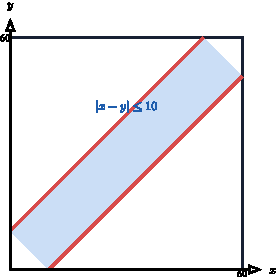
\includegraphics[keepaspectratio,alt={A 60-by-60 arrival-time square with the band abs(x-y) \textless= 10 shaded.}]{assets/notes--fig-prob-01-combinatorics-prob-space-diagram-01.pdf}}

\end{center}

因而概率是

\[{\mathbb{P}}(E) = \frac{m(E)}{m(\Omega)} = \frac{3600 - 2500}{3600} = \frac{11}{36}\]

\end{qlsolution}

\subsection{conditional probability and Bayes' theorem}\label{conditional-probability-and-bayes-theorem}

\begin{definition}{\protect\phantomsection\label{kn-conditional-probability}{\textbf{conditional
probability}}}

对于 probability space \((\Omega,\mathcal{F},{\mathbb{P}})\), 给定一个 event \(B \in \mathcal{F}\), 如果 \({\mathbb{P}}(B) > 0\), 我们定义 conditional probability of an event \(A \in \mathcal{F}\) given \(B\) 为:

\[{\mathbb{P}}(A \mid B) = \frac{{\mathbb{P}}(A \cap B)}{{\mathbb{P}}(B)}\]

\end{definition}

\begin{proposition}{\protect\phantomsection\label{kn-decomposing-probability-of-intersection-of-events}{\textbf{decomposing
probability of intersection of events}}}

令 \(\left( A_{i} \right)_{i \in {\mathbb{N}}}\) 为一个 seq of events, 对于任意 \(n \in {\mathbb{N}}\):

\[{\mathbb{P}}\left( {A_{1} \cap A_{2} \cap \ldots \cap A_{n}} \right) = {\mathbb{P}}\left( A_{1} \right) \cdot {\mathbb{P}}\left( {A_{2} \mid A_{1}} \right) \cdot {\mathbb{P}}\left( {A_{3} \mid A_{1} \cap A_{2}} \right)\ldots \cdot {\mathbb{P}}\left( {A_{n} \mid A_{1} \cap \ldots \cap A_{n - 1}} \right)\]

\end{proposition}

\begin{proof}

Naturally follows from the def.

\end{proof}

\begin{theorem}{\protect\phantomsection\label{kn-law-of-total-probability}{\textbf{law
of total probability}}}

令 \(\left( A_{i} \right)_{i \in {\mathbb{N}}}\) 为一个 seq of \textbf{pairwise disjoint} events, 如果 \(\sqcup_{i = 1}^{\infty}A_{i} = \Omega\), 那么对于任意 event \(E \subseteq \Omega\):

\[{\mathbb{P}}(E) = \sum\limits_{i = 1}^{\infty}{\mathbb{P}}\left( A_{i} \right){\mathbb{P}}\left( {E \mid A_{i}} \right)\]

\end{theorem}

\begin{proof}

\[{\mathbb{P}}(E) = {\mathbb{P}}\left( {E \cap \cup_{i = 1}^{\infty}A_{i}} \right) = {\mathbb{P}}\left( {\cup_{i = 1}^{\infty}E \cap A_{i}} \right) = \sum\limits_{i = 1}^{\infty}{\mathbb{P}}\left( {E \cap A_{i}} \right) = \sum\limits_{i = 1}^{\infty}{\mathbb{P}}\left( A_{i} \right){\mathbb{P}}\left( {E \mid A_{i}} \right)\]

\end{proof}

\begin{qlremark}{Remark}

\(P(A_{i})P(E \mid A_{i})\) 就等于 \(P(E \cap A_{i})\), 也就是在 \(A_{i}\) 这个区域上, \(E\) 的 measure. 因而 disjoint union 之下就是 \(E\) 的完整 measure.

\end{qlremark}

\begin{theorem}{\protect\phantomsection\label{kn-bayes-theorem}{\textbf{Bayes theorem}}}

If \(A,B \subseteq \Omega\) such that \({\mathbb{P}}(B) \neq 0\), then

\[{\mathbb{P}}(A \mid B) = \frac{{\mathbb{P}}(A) \cdot {\mathbb{P}}(B \mid A)}{{\mathbb{P}}(B)}\]

\end{theorem}

\begin{qlremark}{Remark}

这其实是一个非常直接的结果, 因为 \(P(A)\dot{P}(B \mid A) = P(A \cap B)\).\\
但是它的意义在于, 如果我们知道两个事件的概率和其中一个对另一个的条件概率, 我们就也得到了反过来的条件概率.

\end{qlremark}

\begin{example}[(Medical testing)]

在一个群体中, 随机选取一个人患有某种罕见疾病的概率是 0.001. 该疾病有一个诊断测试, 其性质如下: 给定个体患病, 测试呈阳性的概率 (真正阳性率) 是 0.99. 给定个体健康, 测试呈阳性的概率 (假阳性率) 是 0.02. 从群体中随机选取的一个人测试呈阳性. 该个体实际上患有该疾病的概率是多少? 于是

\begin{qlsolution}{Solution}

由 law of total probability, 我们有

\[{\mathbb{P}}(\text{positive}) = {\mathbb{P}}(\text{positive} \mid \text{sick}){\mathbb{P}}(\text{sick}) + {\mathbb{P}}(\text{positive} \mid \text{healthy}){\mathbb{P}}(\text{healthy}) = 0.99 \cdot 0.001 + 0.02 \cdot 0.999 = 0.02097\]

于是

\[{\mathbb{P}}(\text{sick} \mid \text{positive}) = \frac{0.99 \cdot 0.001}{0.02097} \approx 0.047\]

\end{qlsolution}

\end{example}

\begin{example}[(Monty Hall problem)]

假设你参加一个游戏节目, 面前有三扇门: 一扇门后面有一辆车; 其他两扇门后面是山羊. 你选择了一扇门, 比如说是 1 号门, 然后主持人打开了另一扇门, 比如说是 3 号门, 里面有一只山羊. 然后他说 "你想换成 2 号门吗?". 换门对你有利吗?

\begin{qlsolution}{Solution}

令 \(A_{i}\) 表示: car 在 \(i\) 号门后面; \(B\) 事件表示: 主持人打开 3 号门. 我们要求的概率是在事件 \(B\) 发生的情况下, \(A_{2}\) 的个概率, 即 \({\mathbb{P}}(A_{2} \mid B)\). 它的大小是:

\[\begin{matrix}
{{\mathbb{P}}(A_{2} \mid B)} & {= \frac{{\mathbb{P}}(A_{2}) \cdot {\mathbb{P}}(B \mid A_{2})}{{\mathbb{P}}(B)}} \\
 & {= \frac{{\mathbb{P}}(B \mid A_{2}){\mathbb{P}}(A_{2})}{{\mathbb{P}}(B \mid A_{1}){\mathbb{P}}(A_{1}) + {\mathbb{P}}(B \mid A_{2}){\mathbb{P}}(A_{2}) + {\mathbb{P}}(B \mid A_{3}){\mathbb{P}}(A_{3})}} \\
 & {= \frac{1 \cdot \frac{1}{3}}{\frac{1}{2} \cdot \frac{1}{3} + 1 \cdot \frac{1}{3} + 0 \cdot \frac{1}{3}} = \frac{2}{3} > \frac{1}{3}}
\end{matrix}\]

因而, 换门是有利的.

\end{qlsolution}

\begin{qlremark}{Remark}

这是一个非常反直觉的例子. 我们直觉肯定会觉得: 一共 1 辆车和 2 个山羊, 主持人帮忙排除掉了一个山羊, 那么剩下来的两个里面我们二选一, 肯定是 \(1/2\) 概率, 而这个 "更换与否" 就是二选一的抉择. 但其实不是这样的.\\
在第一次选择和第二次选择之间, 主持人带来了额外的信息.

\begin{itemize}
\item
  不换门: win iff 在一开始就选择对了车, 这个概率是 \(1/3\).
\item
  换门: win iff 在一开始选择的是山羊, 这个概率是 \(2/3\).
\end{itemize}

从条件概率的视角来看:

\begin{itemize}
\item
  如果车在 2 号门: 主持人在这个环节里只能选择 3 号门.
\item
  如果车在 1 号门: 主持人在这个环节里可以随机在 2 号和 3 号门里面选择一扇门.
\end{itemize}

也就是说, 主持人打开 3 号门的这个动作, 把 3 号门原本含有的 "中奖潜力" 全部转移给了 2 号门. 这很反直觉. 但是可以用一段 python 程序验证:

\begin{verbatim}
def monty_hall_sim(trials=10000):
    stay_wins = 0
    switch_wins = 0
    for _ in range(trials):
        # 初始化门: 0代表羊, 1代表车
        doors = [0, 0, 0]
        car_position = random.randint(0, 2)
        doors[car_position] = 1

        # 玩家最初的选择
        player_choice = random.randint(0, 2)

        # 主持人打开一扇有山羊的门
        possible_host_doors = [
            i for i in range(3)
            if i != player_choice and doors[i] == 0
        ]
        host_opens = random.choice(possible_host_doors)

        # 如果"不换"赢了
        if doors[player_choice] == 1:
            stay_wins += 1
        # 如果"换门"赢了
        remaining_door = [
            i for i in range(3)
            if i != player_choice and i != host_opens
        ][0]
        if doors[remaining_door] == 1:
            switch_wins += 1
    print(f"坚持不换中奖次数: {stay_wins} (概率: {stay_wins/trials:.2%})")
    print(f"换门后中奖次数: {switch_wins} (概率: {switch_wins/trials:.2%})")
\end{verbatim}

运行结果:

\begin{verbatim}
总实验次数: 10000
坚持不换中奖次数: 3312 (概率: 33.12%)
换门后中奖次数: 6688 (概率: 66.88%)
\end{verbatim}

\end{qlremark}

\end{example}

\begin{example}[(Wizards)]

两个巫师 \(A\) 和 \(B\) 进行决斗, 他们轮流射击对方. 巫师 \(A\) 每次射击命中 \(B\) 的概率是 \({\mathbb{P}}(A) = \frac{1}{2}\), 而巫师 \(B\) 每次射击命中 \(A\) 的概率是 \({\mathbb{P}}(B) = \frac{2}{3}\). 巫师 \(A\) 先开枪. 求: 巫师 \(A\) 获胜的概率是多少?\\

\begin{qlsolution}{Solution}

任意一轮射击 (假设前一轮没有结束, 于是游戏回到初始状态. 因而任意一轮都是独立的) 中, 令 \(W_{A}\) 为事件: \(A\) 获胜; \(W_{B}\) 为事件: \(B\) 获胜, 假设他们从各自开始射击. 根据全概率公式, 我们有

\[\begin{matrix}
 & {{\mathbb{P}}\left( W_{A} \right) = {\mathbb{P}}(hit){\mathbb{P}}\left( {W_{A} \mid hit} \right) + {\mathbb{P}}(miss){\mathbb{P}}\left( {W_{A} \mid miss} \right) = \frac{1}{2} + \frac{1}{2}{\mathbb{P}}\left( W_{B}^{c} \right)} \\
 & {{\mathbb{P}}\left( W_{B} \right) = {\mathbb{P}}(hit){\mathbb{P}}\left( {W_{B} \mid hit} \right) + {\mathbb{P}}(miss){\mathbb{P}}\left( {W_{B} \mid miss} \right) = \frac{2}{3} + \frac{1}{3}{\mathbb{P}}\left( W_{A}^{c} \right)}
\end{matrix}\]

Solving the system, we find \({\mathbb{P}}\left( W_{A} \right) = 0.6\).

\end{qlsolution}

\begin{qlremark}{Remark}

这个例子表明了先手优势有多大. 相比上一个例子, 这是很直观的.\\
另外, 这个例子有趣的是, 我们把无限的回合转化为了一个循环结构, 利用游戏状态的自相似, 只需要考虑任意一轮即可.

\end{qlremark}

\end{example}

\subsection{Kolmogorov definition of conditional probability}\label{kolmogorov-definition-of-conditional-probability}

我们通过 \({\mathbb{P}}(A \mid B) = \frac{{\mathbb{P}}(A \cap B)}{{\mathbb{P}}(B)}\) 定义出来的 conditional probability 有一个限制, 就是 enforce \({\mathbb{P}}(B) > 0\).\\
但是, 难道 \({\mathbb{P}}(B) = 0\) 就不能定义条件概率了吗? 我们考虑一个连续情况: 在 \({\mathbb{R}}^{3}\) 中任意选择一个点, 求: 该点位于单位球面上的概率. 显然, 这个概率是 0. 但是, 如果我们知道该点位于单位球内, 那么该点距离原点的距离为 \(1\) 的概率应当为 \(1\). 也就是说, 即使在 \({\mathbb{P}}(B) = 0\) 的情况下, 我们也希望定义 \({\mathbb{P}}(A \mid B)\).\\
在考虑这个定义之前, 首先我们发现: 基于我们先前定义的 conditional probability, 我们可以获得一个新的 probability space:

\begin{definition}{\protect\phantomsection\label{kn-conditional-probability-space-and-trace-sigma-algebra}{\textbf{conditional
probability space}} and
\protect\phantomsection\label{kn-trace-sigma-algebra}{\textbf{trace
\(\sigma\)-algebra}}}

对于给定的 prob space \((\Omega,\mathcal{F},{\mathbb{P}})\), 给定一个 event \(B \in \mathcal{F}\) 且 \({\mathbb{P}}(B) > 0\), 我们定义 conditional probability space as the triplet \((B,\mathcal{F}_{B},{\mathbb{P}}( \cdot \mid B))\), 其中:

\[F_{B} := \left\{ {A \cap B \mid A \in \mathcal{F}} \right\}\]

继承自原空间的 \href{https://qiulinfan.github.io/qlblog/notes/math/measure-theory/\#kn-sigma-algebra}{\(\sigma\)-algebra} \(\mathcal{F}\), 并被称为 \textbf{trace \(\sigma\)-algebra on \(B\)}.\\
容易验证, 这个 triplet 是一个 prob space.

\end{definition}

\begin{qlremark}{Remark}

当我们把整个 prob space 限制在 event \(B\) 上时, 本质上是在做一个 \href{https://qiulinfan.github.io/qlblog/notes/math/measure-theory/\#kn-radon-nikodym-derivative}{Radon-Nikodym derivative} 的操作.\\
定义 \(f := \frac{{\mathbb{I}}_{B}}{{\mathbb{P}}(B)}\), 那么对于任意 event \(A \in \mathcal{F}_{\mathcal{B}}\), 有:

\[{\mathbb{P}}(A \mid B) = \int_{A}f\, d{\mathbb{P}}\]

因而和我们的直觉一样, 条件概率是通过一个 density function 来重新加权原本的概率测度.

\end{qlremark}

既然这样, 我们能否直接从一个新的 prob space \((B,\mathcal{F}_{B},{\mathbb{P}}( \cdot \mid B))\) 出发, 来定义条件概率呢? 这就是 Kolmogorov 的定义:

\begin{definition}{\protect\phantomsection\label{kn-kolmogorov-definition-of-conditional-probability}{\textbf{Kolmogorov
definition of conditional probability}}}

对于给定的 prob space \((\Omega,\mathcal{F},{\mathbb{P}})\), 设 \(\mathcal{G} \subseteq \mathcal{F}\) 是一个 sub-\(\sigma\)-algebra. 对于 event \(A \in \mathcal{F}\), 条件概率 \({\mathbb{P}}(A \mid \mathcal{G})\) 是一个 \(\mathcal{G}\)-measurable 的随机变量, 其满足对于任意 \(G \in \mathcal{G}\), 有:

\[\int_{G}{\mathbb{P}}(A \mid \mathcal{G})\, d{\mathbb{P}} = {\mathbb{P}}(A \cap G)\]

显然, 当 \({\mathbb{P}}(B) > 0\) 时, 这个定义和我们之前的定义是等价的.\\
这个 random variable \({\mathbb{P}}(A \mid \mathcal{G})\) 在 \(\mathbb{P}\)-a.s. 意义下是唯一的.

\end{definition}

\begin{qlremark}{Remark}

条件概率 \({\mathbb{P}}(A \mid \mathcal{G})\) 这个测度是 \({\mathbb{P}}(A \cap \cdot )\) 这个测度相对于背景测度 \(\mathbb{P}\) 在子信息流 \(\mathcal{G}\) 下的 Radon-Nikodym derivative, 也就是一个密度函数.\\
这个定义里没有指明, 给定一个 event \(B \in \mathcal{F}\), 如何去确定 \(\mathcal{G}\) 以及 \({\mathbb{P}}(A \mid \mathcal{G})\). 虽然这是一个抽象的存在性{ } 唯一性定义, 但是标准的做法是:

\begin{itemize}
\item
  看向产生 \(B\) 的 random variable \(X\), 即 \(B = \left\{ {X = x} \right\}\), 令 \(\mathcal{G} = \sigma(X)\), 即由 random variable \(X\) 生成的 \(\sigma\)-algebra. 这个 \(\sigma\)-algebra 包含了所有关于 \(X\) 可能取值的信息.
\item
  既然 \({\mathbb{P}}(A \mid \sigma(X))\) 是关于 \(\sigma(X)\) 可测的, 那么它一定可以写成 \(h(X)\) 的形式. 通过对 \(X\) 的所有可能取值进行积分, 我们确定了函数 \(h( \cdot )\) 的整体形态, 这时我们定义 \(P(A \mid X = x)\) 为函数 \(h\) 在点 \(x\) 处的值.
\item
  \({\mathbb{P}}(A \mid \mathcal{G})\) 实际就是 \href{https://qiulinfan.github.io/qlblog/notes/math/probability/\#kn-conditional-expectation}{conditional expectation} \({\mathbb{E}}\lbrack{\mathbb{I}}_{A} \mid \mathcal{G}\rbrack\). 当 \({\mathbb{P}}(B) > 0\) 时, 它就退化回经典定义 \(\frac{{\mathbb{P}}(A \cap B)}{{\mathbb{P}}(B)}\).
\end{itemize}

\end{qlremark}

\begin{qlremark}{Remark}

Further issue: \textbf{Borel-Kolmogorov paradox}.\\
即便是这个定义, 也会出现问题.\\
给定一个事件 \(B\), 如果 \({\mathbb{P}}(B) = 0\), 则 \({\mathbb{P}}(A \mid B)\) 的取值取决于我们将 \(B\) 嵌入到哪一个随机变量 \(X\) 中. 不同的随机变量 \(X,Y\) 即使都能产生相同的事件 \(\left\{ {X = x} \right\} = \left\{ {Y = y} \right\} = B\), 它们生成的子 \(\sigma\)-代数 \(\sigma(X)\) 和 \(\sigma(Y)\) 却不同, 导致最终确定的条件概率 \(h_{X}(x) \neq h_{Y}(y)\).\\
为了解决这个问题, 可以引入更精细的结构, 比如说 regular conditional probability, 以及 disintegration theorem. 不过此处不展开了.

\end{qlremark}

\subsection{independence of events}\label{independence-of-events}

\begin{definition}{\protect\phantomsection\label{kn-independence-of-events}{\textbf{independence
of events}}}

对于 prob space \((\Omega,\mathcal{F},{\mathbb{P}})\), 两个 events \(A,B \in \mathcal{F}\) 如果有

\[{\mathbb{P}}(A \cap B) = {\mathbb{P}}(A) \cdot {\mathbb{P}}(B)\]

则称 \(A\) 和 \(B\) 是 independent 的.\\
更加 generally, 对于任意 collection of events \(\left\{ A_{i} \right\}_{i \in I}\), 如果对于任意有限子集 \(J \subseteq I\), 有

\[{\mathbb{P}}\left( {\bigcap\limits_{j \in J}A_{j}} \right) = \prod\limits_{j \in J}{\mathbb{P}}(A_{j})\]

则称 \(\left\{ A_{i} \right\}_{i \in I}\) 是 mutually independent 的.

\end{definition}

\begin{qlremark}{Remark}

根据条件概率的定义, 容易得出: 两个 events \(A,B\) independent 的定义\textbf{等价于 \({\mathbb{P}}(A \mid B) = {\mathbb{P}}(A)\)}, 即事件 \(B\) 的发生与否不影响事件 \(A\) 发生的概率.\\

\begin{proposition}{\protect\phantomsection\label{kn-independence-of-two-events}{\textbf{independence
of two events 的等价定义}}}

对于 prob space \((\Omega,\mathcal{F},{\mathbb{P}})\), 两个 events \(A,B \in \mathcal{F}\) independent iff:

\[{\mathbb{P}}(B \mid A) = {\mathbb{P}}(B)\]

\end{proposition}

\begin{proof}

Directly follows from the definition of conditional probability.

\end{proof}

因而 independence of two events 的定义等价于: 事件 \(A\) 的发生与否不影响事件 \(B\) 发生的概率 (反之亦然).

将它推广到多个事件: 即\textbf{任意一个事件的发生与否都不影响其他事件发生的概率}.

\end{qlremark}

\begin{qlremark}{Remark}

我们从 measure 的角度看待两个事件的 independence: 首先 \({\mathbb{P}}(B) = 0\) 是 trivial case, 而 如果 \({\mathbb{P}}(B) > 0\), 那么 independence 其实可以化为一个等式:

\[\frac{{\mathbb{P}}(A \cap B)}{{\mathbb{P}}(B)} = \frac{{\mathbb{P}}(A)}{{\mathbb{P}}(\Omega)}\]

意思是: 事件 \(A\) 在 \(B\) 这个 set 中占据的 measure 比例, 完全等于事件 \(A\) 在整个空间 \(\Omega\) 中占据的 measure 比例; 也就是说, \textbf{事件 \(B\) 的发生并没有改变事件 \(A\) 在空间中的 measure 分布.}

因而, 这两个集合在 measure (probability) 的意义下是完全解耦的, 这就是 independence 的 information geometric 意义.

\end{qlremark}

\begin{proposition}

如果 events \(A\) 和 \(B\) independent, 则 \(A\) 和 \(B^{c}\) 也是 independent 的.

\end{proposition}

\begin{proof}

\[\begin{matrix}
{{\mathbb{P}}\left( {A^{c} \cap B^{c}} \right)} & {= {\mathbb{P}}\left( {(A \cup B)^{c}} \right) = 1 - {\mathbb{P}}(A \cup B) = 1 - {\mathbb{P}}(A) - {\mathbb{P}}(B) + {\mathbb{P}}(A \cap B)} \\
 & {= 1 - {\mathbb{P}}(A) - {\mathbb{P}}(B) + {\mathbb{P}}(A) \cdot {\mathbb{P}}(B) = (1 - {\mathbb{P}}(A))(1 - {\mathbb{P}}(B))} \\
 & {= {\mathbb{P}}\left( A^{c} \right) \cdot {\mathbb{P}}\left( B^{c} \right)}
\end{matrix}\]

\end{proof}

\begin{example}[(Pairwise Independence vs. Mutual Independence)]

一组事件 \(A_{1},A_{2},\ldots \in \mathcal{F}\) 如果是 mutually independent 的, 则它们两两 independent. \textbf{但是反过来不成立}.\\
即: \textbf{即便对于任意 \(i \neq j\), 有 \({\mathbb{P}}(A_{i} \cap A_{j}) = {\mathbb{P}}(A_{i}){\mathbb{P}}(A_{j})\), 也并不意味着这些事件是 mutually independent 的}.\\
下面为一个 counterexample: 考虑掷两个骰子. 令事件

\[A := \left\{ {\text{first roll is}\ 4} \right\},\quad B := \left\{ {\text{second roll is}\ 3} \right\},\quad C := \left\{ {\text{the sum of the two outcomes is}\ 7} \right\}\]

我们发现: \({\mathbb{P}}(A \cap B \cap C) = \frac{1}{36} \neq {\mathbb{P}}(A){\mathbb{P}}(B){\mathbb{P}}(C) = \frac{1}{6^{3}}\), 因而 \(A,B,C\) 并不 mutually independent. 然而, However, \({\mathbb{P}}(A \cap B) = \frac{1}{36} = {\mathbb{P}}(A){\mathbb{P}}(B),{\mathbb{P}}(A \cap C) = \frac{1}{36} = {\mathbb{P}}(A){\mathbb{P}}(C)\) and \({\mathbb{P}}(B \cap C) = \frac{1}{36} = {\mathbb{P}}(B){\mathbb{P}}(C)\), 因而它们两两 pairwise independent.

\end{example}

\begin{qlremark}{Remark}

这个反例能够成功的理由是: 事件 \(C\) (总和) 和 事件 \(A\) (第一个骰子) 以及事件 \(B\) (第二个骰子) 分别都是独立的, 因为知道了其中一个并不会影响另一个的概率. 但是, 一旦我们知道了 \(A\) 和 \(B\) 的值, 那么 \(C\) 的值就被完全确定了 (因为总和就是两个骰子的和). 因而, 三个事件并不 mutually independent.\\
(注意: 如果 \(C\) 事件不是和为 7 而是一个小于 7 的数, 那就不是了, 因为如果我们知道第一次是 6, 那么和就不可能是 6, 那么就也失去了 pairwise independence).\\
这个例子说明了, mutual independence 是一个比较强的条件. 我们可以把这三个事件看作是对结果空间的约束:

\begin{itemize}
\item
  两个骰子的结果空间有 36 个点.
\item
  \(A\) 是一条线 (6个点), \(B\) 是另一条线 (6个点), \(C\) 是一条对角线 (6个点)。
\item
  两两独立: 意味着任意两条线相交的点数, 恰好符合概率乘积.
\item
  相互独立: 要求这三条线交于一点的概率也符合乘积.
\end{itemize}

这个例子提醒我们: 独立性不是一种可以由低维向高维简单``归纳''的性质. 一个系统可以局部解耦（两两独立, 但在全局尺度上却存在强耦合. 总之 mutual independence 是一个很强的条件.

\end{qlremark}

\begin{example}[(coin tossing)]

假设我们有一枚不均匀的硬币, 掷出正面的概率是 \(p \in \lbrack 0,1\rbrack\), 反面的概率是 \(1 - p\). 我们不断地掷这枚硬币, 直到第一次掷出正面为止, 并记录所需的掷币次数. 求: 掷币次数为奇数的概率是多少?

\begin{qlsolution}{Solution}

对于任意 \(i \in {\mathbb{N}}\), 考虑事件 \(A_{i} = \{\) 掷币次数为 \(i\}\).

\[{\mathbb{P}}\left( {\cup_{n = 1}^{\infty}A_{2n - 1}} \right) = \sum\limits_{n = 1}^{\infty}{\mathbb{P}}\left( A_{2n - 1} \right) = \sum\limits_{n = 1}^{\infty}(1 - p)^{2n - 2}p = p\sum\limits_{n = 1}^{\infty}\left( {(1 - p)^{2}} \right)^{n - 1} = p \cdot \frac{1}{1 - (1 - p)^{2}} = \frac{1}{2 - p}\]

\end{qlsolution}

\begin{qlremark}{Remark}

这个问题还可以通过 law of total probability 来解决.\\
令 \(E =\) 掷币次数为奇数. 那么

\[\begin{matrix}
{{\mathbb{P}}(E)} & {= {\mathbb{P}}(\text{head}) \cdot {\mathbb{P}}(E \mid \text{head}) + {\mathbb{P}}(\text{tail}) \cdot {\mathbb{P}}(E \mid \text{tail})} \\
 & {= p \cdot 1 + (1 - p) \cdot (1 - {\mathbb{P}}(E))}
\end{matrix}\]

Solve 这个 equation 得到同样结果.

\end{qlremark}

\end{example}
\end{document}
